\chapter{Технологийн судалгаа}
\section{BLoC}
"Hoome" платформын мобайл аппликейшн нь програмчлалын Dart хэл буюу Flutter технологийг ашиглан бичигдсэн бөгөөд түүн дотроо төлвийн менежмент сан болох BLoC(Business Logic Components)-ийг ашигладаг. 

BLoC нь хэрэглэгчийн интерфейсийг бизнес логикоос тусгаарлаж өгөх зорилготой сан бөгөөд event-driven архитектур дээр суурилсан байдаг. 

BLoC нь таны Flutter програмын төлвийг удирдах, хэрэглэгчийн харилцан үйлчлэлийг бүтэцтэй байдлаар зохицуулах design pattern юм. Энэ нь апп доторх data stream болон удирдахын тулд event, stream-ийн тухай ойлголтыг ашигладаг.

Flutter BLoC технологи нь:

\begin{enumerate}
  \item \textbf{Events}: Event нь хэрэглэгчийн аппликейшнд үзүүлэх ямарваа нэгэн хариу үйлдэл бөгөөд тухайн event-ийг BLoC компонент хүлээн авч, логик үйлдлүүдийг хийж боловсруулснаар одоо байгаа төлвүүдийг шинэчилж шинэ төлвийг үүсгэдэг.
  \item \textbf{BLoC Component}: Event-үүдийг сонсож, утга хүлээн авахад үргэлж бэлэн байдаг бөгөөд event-үүд нь өөрийн утгатай байх боломжтой. Хүлээн авсан эвентүүдийг хэрэглэгчийн интерфейст ашиглагдаж буй төлөв, төлвийн өгөгдлийг шинэчлэхэд ашигладаг.
  \item \textbf{Streams}: Event-үүд нь ихэвчлэн stream байдлаар хадгалагдаж, орсон дарааллаараа ачаалладаг бөгөөд BLoC компонентүүд нь тус бүр өөрийн зааж өгсөн урсгалыг сонсож байдаг.
  \item \textbf{States}: Аппликейшн дээр ашиглагдаж буй бүх төрлийн датаг state буюу төлөв гэж нэрэлж байгаа бөгөөд тухайн төлөв нь BLoC компонентоор дамжуулагдан шинэчлэгдэж, улмаар хэрэглэгчийн интерфейст өөрчлөлт ороход хүргэдэг. 
\end{enumerate}

Эдгээр 4 үндсэн элементүүдээс бүрдэх бөгөөд хэрэглэгчийн интерфейст шинэчлэл хийх, өөрчлөлт оруулах үед интерфесийн логикоос хамааран онцгой тохиолдол(exception), алдаа(runtime error)-наас сэргийлэх боломжтой. Аппликейшнийн usability болон scalability-г илүү амар хялбар байдлаар хангаж өгдөг сан юм. 

\begin{figure}
  \centering
  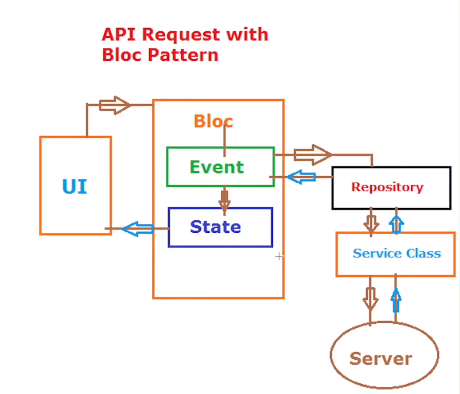
\includegraphics[scale=0.5]{imgs/bloc.png}
  \caption{BLoC }
\end{figure}

